%========== naive_bayes.tex ==========

\section{Naive Bayes Classifier}

\subsection{Motivation}

\begin{frame}{Bayes Decision Theory}
\begin{itemize}
    \item Given a dataset: $\{(x^{(i)}, y^{(i)})\}_{i=1}^m$
    \item Each sample: $x^{(i)} \in \R^n$ with features $x^{(i)} = (x^{(i)}_1, \ldots, x^{(i)}_n)$
    \item Labels: $y^{(i)} \in \{1, 2, \ldots, K\}$
    \pause
    \item \textbf{Bayes optimal classifier} minimizes expected risk:
    \[
    \hat{y} = \argmax_{k \in \{1,\ldots,K\}} P(y = k \mid x)
    \]
    \pause
    \item Using Bayes' rule:
    \[
    P(y = k \mid x) = \frac{P(x \mid y = k) P(y = k)}{P(x)}
    \]
    \pause
    \item Since $P(x)$ is constant for all classes:
    \[
    \hat{y} = \argmax_{k} P(x \mid y = k) P(y = k)
    \]
\end{itemize}
\end{frame}

\begin{frame}{The Challenge: High-Dimensional Likelihood}
\begin{itemize}
    \item To compute $P(x \mid y = k)$, we need:
    \[
    P(x_1, x_2, \ldots, x_n \mid y = k)
    \]
    \pause
    \item For $n$ features, this requires estimating:
    \begin{itemize}
        \item Joint distribution over $n$ variables
        \item Exponential number of parameters: $O(|\text{domain}|^n)$
    \end{itemize}
    \pause
    \item \textbf{Example:} Binary features, $n=100$ $\Rightarrow$ $2^{100}$ parameters per class!
    \pause
    \item \textbf{Solution:} Make a simplifying assumption...
\end{itemize}
\end{frame}

\subsection{The Naive Bayes Assumption}

\begin{frame}{Conditional Independence}
\begin{definition}[Naive Bayes Assumption]
Given the class label $y$, features are conditionally independent:
\[
P(x_1, x_2, \ldots, x_n \mid y = k) = \prod_{j=1}^n P(x_j \mid y = k)
\]
\end{definition}
\pause
\begin{itemize}
    \item \textbf{"Naive"} because this assumption is rarely true in practice
    \item But it works surprisingly well!
    \pause
    \item Reduces parameter count from $O(|\text{domain}|^n)$ to $O(n \cdot |\text{domain}|)$
    \pause
    \item Each feature's distribution is estimated independently
\end{itemize}
\end{frame}

\begin{frame}{MAP Decision Rule}
\begin{itemize}
    \item With the naive assumption:
    \[
    P(y = k \mid x) \propto P(y = k) \prod_{j=1}^n P(x_j \mid y = k)
    \]
    \pause
    \item Define:
    \begin{itemize}
        \item Class prior: $\pi_k = P(y = k)$
        \item Class-conditional likelihood: $P(x_j \mid y = k)$
    \end{itemize}
    \pause
    \item MAP prediction:
    \[
    \hat{y} = \argmax_{k \in \{1,\ldots,K\}} \pi_k \prod_{j=1}^n P(x_j \mid y = k)
    \]
\end{itemize}
\end{frame}

\begin{frame}{Log-Space MAP Rule (Derivation)}
\begin{itemize}
    \item Working in log-space avoids numerical underflow:
    \pause
    \begin{align*}
    \hat{y} &= \argmax_{k} \pi_k \prod_{j=1}^n P(x_j \mid y = k) \\
    \pause
    &= \argmax_{k} \log\left(\pi_k \prod_{j=1}^n P(x_j \mid y = k)\right) \\
    \pause
    &= \argmax_{k} \left[\log \pi_k + \sum_{j=1}^n \log P(x_j \mid y = k)\right]
    \end{align*}
    \pause
    \item \textbf{Final prediction rule:}
    \[
    \hat{y} = \argmax_{k} \left[\log \pi_k + \sum_{j=1}^n \log P(x_j \mid y = k)\right]
    \]
    \pause
    \item This is the form we use in practice!
\end{itemize}
\end{frame}

\subsection{Parameter Estimation}

\begin{frame}{Estimating Class Priors}
\begin{itemize}
    \item Maximum Likelihood Estimate (MLE):
    \[
    \hat{\pi}_k = \frac{\text{count}(y = k)}{m} = \frac{1}{m} \sum_{i=1}^m \mathbf{1}[y^{(i)} = k]
    \]
    \pause
    \item Maximum A Posteriori (MAP) with Dirichlet prior:
    \[
    \hat{\pi}_k = \frac{\text{count}(y = k) + \alpha_k}{m + \sum_{k'=1}^K \alpha_{k'}}
    \]
    \pause
    \item For uniform prior ($\alpha_k = 1$ for all $k$):
    \[
    \hat{\pi}_k = \frac{\text{count}(y = k) + 1}{m + K}
    \]
\end{itemize}
\end{frame}

\begin{frame}{Gaussian Naive Bayes}
\begin{itemize}
    \item For continuous features, assume:
    \[
    P(x_j \mid y = k) = \mathcal{N}(x_j; \mu_{kj}, \sigma_{kj}^2)
    \]
    \pause
    \item Parameters per class $k$ and feature $j$:
    \begin{itemize}
        \item Mean: $\mu_{kj} = \E[x_j \mid y = k]$
        \item Variance: $\sigma_{kj}^2 = \Var[x_j \mid y = k]$
    \end{itemize}
    \pause
    \item MLE estimates:
    \[
    \hat{\mu}_{kj} = \frac{1}{m_k} \sum_{i: y^{(i)} = k} x_j^{(i)}
    \]
    \[
    \hat{\sigma}_{kj}^2 = \frac{1}{m_k} \sum_{i: y^{(i)} = k} (x_j^{(i)} - \hat{\mu}_{kj})^2
    \]
    where $m_k = \text{count}(y = k)$
\end{itemize}
\end{frame}

\begin{frame}{Multinomial Naive Bayes}
\begin{itemize}
    \item For discrete/count features (e.g., word counts):
    \[
    P(x_j = v \mid y = k) = \theta_{kv}
    \]
    where $\sum_v \theta_{kv} = 1$
    \pause
    \item MLE estimate:
    \[
    \hat{\theta}_{kv} = \frac{\text{count}(x_j = v, y = k)}{\text{count}(y = k)}
    \]
    \pause
    \item \textbf{Zero-frequency problem:} If $x_j = v$ never appears in class $k$, then $\hat{\theta}_{kv} = 0$
    \pause
    \item This makes $\log P(x_j = v \mid y = k) = -\infty$ for any test sample!
\end{itemize}
\end{frame}

\begin{frame}{Laplace Smoothing (Add-$\alpha$)}
\begin{itemize}
    \item Add pseudocounts to avoid zero probabilities:
    \[
    \hat{\theta}_{kv} = \frac{\text{count}(x_j = v, y = k) + \alpha}{\text{count}(y = k) + \alpha \cdot |V_j|}
    \]
    \pause
    \item Common choice: $\alpha = 1$ (Laplace smoothing)
    \pause
    \item Interpretation: Bayesian MAP with Dirichlet prior
    \pause
    \item Ensures: $\hat{\theta}_{kv} > 0$ for all $v, k$
    \pause
    \item In log-space: $\log \hat{\theta}_{kv} > -\infty$
\end{itemize}
\end{frame}

\begin{frame}{Bernoulli Naive Bayes}
\begin{itemize}
    \item For binary features (e.g., word presence/absence):
    \[
    P(x_j = 1 \mid y = k) = p_{kj}
    \]
    \pause
    \item MLE with smoothing:
    \[
    \hat{p}_{kj} = \frac{\text{count}(x_j = 1, y = k) + \alpha}{\text{count}(y = k) + 2\alpha}
    \]
    \pause
    \item Probability mass function:
    \[
    P(x_j \mid y = k) = \hat{p}_{kj}^{x_j} (1 - \hat{p}_{kj})^{1-x_j}
    \]
    \pause
    \item In log-space:
    \[
    \log P(x_j \mid y = k) = x_j \log \hat{p}_{kj} + (1-x_j) \log(1 - \hat{p}_{kj})
    \]
\end{itemize}
\end{frame}

\subsection{Worked Examples}

\begin{frame}{Example 1: Gaussian Naive Bayes (1D)}
\textbf{Problem:} Classify height (in cm) into two classes: Child ($y=1$) and Adult ($y=2$)

\textbf{Training data:}
\begin{itemize}
    \item Children: $[100, 110, 105, 115, 108]$
    \item Adults: $[170, 175, 180, 165, 172]$
\end{itemize}
\pause
\textbf{Estimate parameters:}
\begin{itemize}
    \item $\hat{\pi}_1 = 5/10 = 0.5$, $\hat{\pi}_2 = 5/10 = 0.5$
    \pause
    \item Class 1: $\hat{\mu}_1 = 107.6$, $\hat{\sigma}_1^2 = 31.04$
    \item Class 2: $\hat{\mu}_2 = 172.4$, $\hat{\sigma}_2^2 = 32.24$
\end{itemize}
\pause
\textbf{Predict:} $x = 120$ cm
\begin{align*}
\text{Score}_1 &= \log 0.5 + \log \mathcal{N}(120; 107.6, 31.04) \approx -0.693 - 2.33 = -3.02 \\
\text{Score}_2 &= \log 0.5 + \log \mathcal{N}(120; 172.4, 32.24) \approx -0.693 - 41.5 = -42.2
\end{align*}
\pause
$\hat{y} = 1$ (Child) ✓
\end{frame}

\begin{frame}{Example 1: Visualization}
\begin{center}
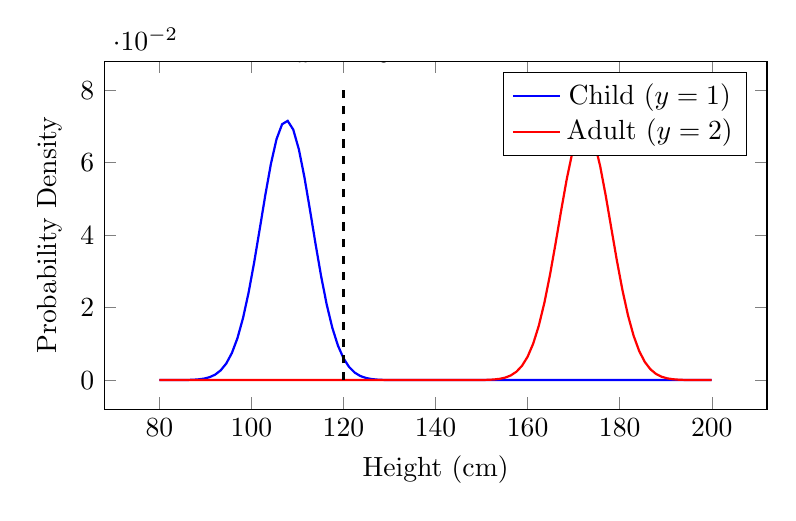
\begin{tikzpicture}
\begin{axis}[
    width=10cm,
    height=6cm,
    xlabel={Height (cm)},
    ylabel={Probability Density},
    legend pos=north east,
    domain=80:200,
    samples=100
]
\addplot[blue, thick] {exp(-0.5*((x-107.6)^2)/31.04) / sqrt(2*pi*31.04)};
\addlegendentry{Child ($y=1$)}
\addplot[red, thick] {exp(-0.5*((x-172.4)^2)/32.24) / sqrt(2*pi*32.24)};
\addlegendentry{Adult ($y=2$)}
\addplot[black, dashed, thick] coordinates {(120,0) (120,0.08)};
\node at (axis cs:120,0.09) {$x=120$};
\end{axis}
\end{tikzpicture}
\end{center}
\pause
\begin{itemize}
    \item Decision boundary: where $P(y=1 \mid x) = P(y=2 \mid x)$
    \item Approximately at $x \approx 140$ cm
\end{itemize}
\end{frame}

\begin{frame}{Example 2: Multinomial Naive Bayes (Text)}
\textbf{Problem:} Classify documents as Spam ($y=1$) or Ham ($y=2$)

\textbf{Vocabulary:} $\{\text{"buy"}, \text{"cheap"}, \text{"meeting"}, \text{"tomorrow"}\}$

\textbf{Training data:}
\begin{itemize}
    \item Spam: "buy cheap", "buy buy cheap"
    \item Ham: "meeting tomorrow", "meeting meeting tomorrow"
\end{itemize}
\pause
\textbf{Estimate parameters (with $\alpha=1$):}
\begin{itemize}
    \item $\hat{\pi}_1 = 0.5$, $\hat{\pi}_2 = 0.5$
    \pause
    \item For Spam ($y=1$):
    \begin{itemize}
        \item "buy": count=3, $\hat{\theta}_{1,\text{buy}} = (3+1)/(6+4) = 0.4$
        \item "cheap": count=2, $\hat{\theta}_{1,\text{cheap}} = (2+1)/(6+4) = 0.3$
        \item "meeting": count=0, $\hat{\theta}_{1,\text{meeting}} = (0+1)/(6+4) = 0.1$
        \item "tomorrow": count=0, $\hat{\theta}_{1,\text{tomorrow}} = (0+1)/(6+4) = 0.1$
    \end{itemize}
\end{itemize}
\end{frame}

\begin{frame}{Example 2: Multinomial NB (continued)}
\textbf{For Ham ($y=2$):}
\begin{itemize}
    \item "buy": count=0, $\hat{\theta}_{2,\text{buy}} = (0+1)/(6+4) = 0.1$
    \item "cheap": count=0, $\hat{\theta}_{2,\text{cheap}} = (0+1)/(6+4) = 0.1$
    \item "meeting": count=3, $\hat{\theta}_{2,\text{meeting}} = (3+1)/(6+4) = 0.4$
    \item "tomorrow": count=2, $\hat{\theta}_{2,\text{tomorrow}} = (2+1)/(6+4) = 0.3$
\end{itemize}
\pause
\textbf{Predict:} "buy cheap meeting"
\begin{align*}
\text{Score}_1 &= \log 0.5 + \log 0.4 + \log 0.3 + \log 0.1 \\
             &= -0.693 - 0.916 - 1.204 - 2.303 = -5.116 \\
\text{Score}_2 &= \log 0.5 + \log 0.1 + \log 0.1 + \log 0.4 \\
             &= -0.693 - 2.303 - 2.303 - 0.916 = -6.215
\end{align*}
\pause
$\hat{y} = 1$ (Spam) ✓
\end{frame}

\begin{frame}{Example 3: 2D Gaussian Naive Bayes}
\begin{center}
\begin{tikzpicture}
\begin{axis}[
    width=10cm,
    height=8cm,
    xlabel={$x_1$},
    ylabel={$x_2$},
    legend pos=north east,
    domain=-2:6,
    y domain=-2:6,
    view={0}{90}
]
% Class 1: mean (1,1), cov diag(1,1)
\addplot3[contour filled={levels={0.01,0.05,0.1,0.15,0.2}},blue,opacity=0.3] 
    {exp(-0.5*((x-1)^2 + (y-1)^2)) / (2*pi)};
% Class 2: mean (4,4), cov diag(1,1)
\addplot3[contour filled={levels={0.01,0.05,0.1,0.15,0.2}},red,opacity=0.3] 
    {exp(-0.5*((x-4)^2 + (y-4)^2)) / (2*pi)};
% Decision boundary (linear in this case)
\addplot[black, dashed, thick] coordinates {(2.5,-1) (2.5,6)};
\node at (axis cs:2.5,5.5) {Decision boundary};
% Sample points
\addplot[only marks, mark=*, blue, mark size=2pt] coordinates {
    (0.5,0.8) (1.2,1.1) (0.9,1.3) (1.1,0.7)
};
\addplot[only marks, mark=*, red, mark size=2pt] coordinates {
    (3.8,4.1) (4.2,3.9) (4.0,4.3) (3.9,4.0)
};
\end{axis}
\end{tikzpicture}
\end{center}
\pause
\begin{itemize}
    \item With independent features, decision boundary is linear
    \item For Gaussian NB with equal variances, boundary is a hyperplane
\end{itemize}
\end{frame}

\subsection{Algorithms}

\begin{frame}{Training Algorithm (Gaussian NB)}
\begin{algorithm}[H]
\SetAlgoLined
\KwIn{Training set $\{(x^{(i)}, y^{(i)})\}_{i=1}^m$}
\KwOut{Parameters: $\{\hat{\pi}_k, \hat{\mu}_{kj}, \hat{\sigma}_{kj}^2\}$}
\BlankLine
\For{$k = 1$ \textbf{to} $K$}{
    $m_k \leftarrow \sum_{i=1}^m \mathbf{1}[y^{(i)} = k]$ \\
    $\hat{\pi}_k \leftarrow m_k / m$ \\
    \For{$j = 1$ \textbf{to} $n$}{
        $\hat{\mu}_{kj} \leftarrow \frac{1}{m_k} \sum_{i: y^{(i)} = k} x_j^{(i)}$ \\
        $\hat{\sigma}_{kj}^2 \leftarrow \frac{1}{m_k} \sum_{i: y^{(i)} = k} (x_j^{(i)} - \hat{\mu}_{kj})^2$
    }
}
\end{algorithm}
\pause
\textbf{Complexity:} $O(m \cdot n)$ time, $O(K \cdot n)$ space
\end{frame}

\begin{frame}{Prediction Algorithm (Log-Space MAP)}
\begin{algorithm}[H]
\SetAlgoLined
\KwIn{Test sample $x$, parameters $\{\hat{\pi}_k, \hat{\mu}_{kj}, \hat{\sigma}_{kj}^2\}$}
\KwOut{Predicted class $\hat{y}$}
\BlankLine
\For{$k = 1$ \textbf{to} $K$}{
    $\text{score}_k \leftarrow \log \hat{\pi}_k$ \\
    \For{$j = 1$ \textbf{to} $n$}{
        $\text{score}_k \leftarrow \text{score}_k + \log \mathcal{N}(x_j; \hat{\mu}_{kj}, \hat{\sigma}_{kj}^2)$
    }
}
$\hat{y} \leftarrow \argmax_{k} \text{score}_k$
\end{algorithm}
\pause
\textbf{Complexity:} $O(K \cdot n)$ time per prediction
\end{frame}

\subsection{Conceptual Understanding}

\begin{frame}{Generative vs Discriminative Models}
\begin{columns}
\begin{column}{0.5\textwidth}
\textbf{Generative (Naive Bayes)}
\begin{itemize}
    \item Models $P(x, y) = P(y) P(x \mid y)$
    \item Learns class-conditional distributions
    \item Can generate new samples
    \item Requires independence assumptions
    \item Works well with small data
\end{itemize}
\end{column}
\pause
\begin{column}{0.5\textwidth}
\textbf{Discriminative (Logistic Regression)}
\begin{itemize}
    \item Models $P(y \mid x)$ directly
    \item Learns decision boundary
    \item Cannot generate samples
    \item Fewer assumptions
    \item Often better with large data
\end{itemize}
\end{column}
\end{columns}
\pause
\vspace{0.5cm}
\textbf{Key insight:} Naive Bayes is a generative model that makes strong independence assumptions to make learning tractable.
\end{frame}

\begin{frame}{Relationship to Logistic Regression}
\begin{itemize}
    \item Under Gaussian NB with shared variance, the decision boundary is:
    \[
    \log \frac{P(y=1 \mid x)}{P(y=2 \mid x)} = w_0 + \sum_{j=1}^n w_j x_j
    \]
    \pause
    \item This is exactly the form of logistic regression!
    \pause
    \item \textbf{Difference:}
    \begin{itemize}
        \item NB: Parameters come from MLE of class-conditional distributions
        \item LR: Parameters optimized to maximize conditional likelihood
    \end{itemize}
    \pause
    \item \textbf{When features are truly independent:} NB and LR learn similar boundaries
    \item \textbf{When features are correlated:} LR typically performs better
\end{itemize}
\end{frame}

\subsection{Practical Considerations}

\begin{frame}{Overconfidence and Calibration}
\begin{itemize}
    \item Naive Bayes often produces \textbf{overconfident} probabilities
    \pause
    \item Example: $P(y=k \mid x) = 0.99$ when true probability might be $0.7$
    \pause
    \item \textbf{Causes:}
    \begin{itemize}
        \item Independence assumption is violated
        \item Features are multiplied, amplifying errors
        \item MLE estimates can be extreme
    \end{itemize}
    \pause
    \item \textbf{Solutions:}
    \begin{itemize}
        \item Use Platt scaling or isotonic regression for calibration
        \item Use temperature scaling: $P_{\text{cal}}(y \mid x) \propto P(y \mid x)^{1/T}$
        \item For classification, overconfidence may not matter (only argmax matters)
    \end{itemize}
\end{itemize}
\end{frame}

\begin{frame}{Computational Complexity}
\begin{itemize}
    \item \textbf{Training:} $O(m \cdot n)$
    \begin{itemize}
        \item One pass through data
        \item Compute means/variances per class-feature pair
    \end{itemize}
    \pause
    \item \textbf{Prediction:} $O(K \cdot n)$ per sample
    \begin{itemize}
        \item Evaluate $K$ classes, $n$ features each
        \item Very fast!
    \end{itemize}
    \pause
    \item \textbf{Storage:} $O(K \cdot n)$ parameters
    \begin{itemize}
        \item Gaussian NB: $2Kn$ (means + variances)
        \item Multinomial NB: $Kn|V|$ (vocabulary size dependent)
    \end{itemize}
    \pause
    \item \textbf{Advantage:} Extremely efficient for high-dimensional sparse data (e.g., text)
\end{itemize}
\end{frame}

\begin{frame}{Common Mistakes}
\begin{enumerate}
    \item \textbf{Forgetting log-space:} Multiplying probabilities causes underflow
    \pause
    \item \textbf{Zero-frequency problem:} Not using smoothing for discrete features
    \pause
    \item \textbf{Feature scaling:} Gaussian NB assumes features are on similar scales
    \pause
    \item \textbf{Continuous features with Multinomial NB:} Wrong model choice
    \pause
    \item \textbf{Assuming independence holds:} Features are often correlated
    \pause
    \item \textbf{Using test data for parameter estimation:} Data leakage!
    \pause
    \item \textbf{Not handling missing features:} Need to skip or impute
\end{enumerate}
\end{frame}

\subsection{Exercises}

\begin{frame}{Exercise 1: Basic Probability}
Given: $P(y=1) = 0.6$, $P(x_1=1 \mid y=1) = 0.8$, $P(x_1=1 \mid y=2) = 0.3$

Compute: $P(y=1 \mid x_1=1)$

\vspace{0.5cm}
\pause
\textbf{Solution:}
\[
P(y=1 \mid x_1=1) = \frac{0.6 \times 0.8}{0.6 \times 0.8 + 0.4 \times 0.3} = \frac{0.48}{0.48 + 0.12} = 0.8
\]
\end{frame}

\begin{frame}{Exercise 2: Log-Space Computation}
Given: $\pi_1 = 0.7$, $P(x_1=1 \mid y=1) = 0.9$, $P(x_2=0 \mid y=1) = 0.2$

Compute log-score for class 1: $\log \pi_1 + \log P(x_1=1 \mid y=1) + \log P(x_2=0 \mid y=1)$

\vspace{0.5cm}
\pause
\textbf{Solution:}
\[
\log 0.7 + \log 0.9 + \log 0.2 = -0.357 - 0.105 - 1.609 = -2.071
\]
\end{frame}

\begin{frame}{Exercise 3: Parameter Estimation}
Training data: $y^{(1)}=1, y^{(2)}=1, y^{(3)}=2, y^{(4)}=2, y^{(5)}=2$

Estimate: $\hat{\pi}_1$ and $\hat{\pi}_2$ using MLE

\vspace{0.5cm}
\pause
\textbf{Solution:}
\[
\hat{\pi}_1 = \frac{2}{5} = 0.4, \quad \hat{\pi}_2 = \frac{3}{5} = 0.6
\]
\end{frame}

\begin{frame}{Exercise 4: Gaussian MLE}
Class 1 samples for feature $j$: $[2, 4, 3, 5]$

Estimate: $\hat{\mu}_{1j}$ and $\hat{\sigma}_{1j}^2$

\vspace{0.5cm}
\pause
\textbf{Solution:}
\[
\hat{\mu}_{1j} = \frac{2+4+3+5}{4} = 3.5
\]
\[
\hat{\sigma}_{1j}^2 = \frac{(2-3.5)^2 + (4-3.5)^2 + (3-3.5)^2 + (5-3.5)^2}{4} = 1.25
\]
\end{frame}

\begin{frame}{Exercise 5: Laplace Smoothing}
Vocabulary size $|V|=10$, class $k$ has 5 word tokens total, word "hello" appears 2 times.

Estimate $\hat{\theta}_{k,\text{hello}}$ with $\alpha=1$

\vspace{0.5cm}
\pause
\textbf{Solution:}
\[
\hat{\theta}_{k,\text{hello}} = \frac{2 + 1}{5 + 1 \times 10} = \frac{3}{15} = 0.2
\]
\end{frame}

\begin{frame}{Exercise 6: Decision Boundary}
Gaussian NB with:
\begin{itemize}
    \item Class 1: $\mu_1 = 0$, $\sigma_1^2 = 1$, $\pi_1 = 0.5$
    \item Class 2: $\mu_2 = 2$, $\sigma_2^2 = 1$, $\pi_2 = 0.5$
\end{itemize}

Find the decision boundary (where $P(y=1 \mid x) = P(y=2 \mid x)$)

\vspace{0.5cm}
\pause
\textbf{Solution:}
\[
\log 0.5 - \frac{(x-0)^2}{2} = \log 0.5 - \frac{(x-2)^2}{2}
\]
\[
x^2 = (x-2)^2 \Rightarrow x = 1
\]
Decision boundary at $x = 1$
\end{frame}

\begin{frame}{Exercise 7: Bernoulli NB}
Binary features: $x_1, x_2 \in \{0,1\}$

Training: $(x_1=1, x_2=0, y=1)$ appears 3 times, $(x_1=0, x_2=1, y=1)$ appears 2 times

Estimate $P(x_1=1 \mid y=1)$ and $P(x_2=1 \mid y=1)$ with $\alpha=1$

\vspace{0.5cm}
\pause
\textbf{Solution:}
\[
P(x_1=1 \mid y=1) = \frac{3 + 1}{5 + 2} = \frac{4}{7} \approx 0.571
\]
\[
P(x_2=1 \mid y=1) = \frac{2 + 1}{5 + 2} = \frac{3}{7} \approx 0.429
\]
\end{frame}

\begin{frame}{Exercise 8: Feature Independence}
True or False: If features $x_1$ and $x_2$ are correlated in the data, Naive Bayes will still work correctly because it assumes independence.

\vspace{0.5cm}
\pause
\textbf{Solution:} False. Naive Bayes will still make predictions, but the independence assumption violation means:
\begin{itemize}
    \item Probability estimates will be inaccurate
    \item Performance may degrade compared to models that account for correlations
    \item However, NB can still work well in practice despite violations
\end{itemize}
\end{frame}

\begin{frame}{Exercise 9: Computational Cost}
Dataset: $m=10^6$ samples, $n=1000$ features, $K=10$ classes

Estimate training time complexity and prediction time per sample.

\vspace{0.5cm}
\pause
\textbf{Solution:}
\begin{itemize}
    \item Training: $O(m \cdot n) = O(10^9)$ operations
    \item Prediction: $O(K \cdot n) = O(10^4)$ operations per sample
    \item Very efficient for prediction!
\end{itemize}
\end{frame}

\begin{frame}{Exercise 10: Zero Probability Problem}
Without smoothing, if a test sample contains word "xyz" that never appeared in class $k$ during training, what happens to $\log P(\text{"xyz"} \mid y=k)$?

\vspace{0.5cm}
\pause
\textbf{Solution:}
\[
\hat{\theta}_{k,\text{xyz}} = 0 \Rightarrow \log 0 = -\infty
\]
This makes the entire log-score $-\infty$ for class $k$, regardless of other features. This is why smoothing is essential!
\end{frame}

\subsection{Summary}

\begin{frame}{Summary: Naive Bayes Classifier}
\begin{itemize}
    \item \textbf{Core idea:} Use Bayes' rule with conditional independence assumption
    \pause
    \item \textbf{Prediction:} $\hat{y} = \argmax_k [\log \pi_k + \sum_{j=1}^n \log P(x_j \mid y=k)]$
    \pause
    \item \textbf{Variants:}
    \begin{itemize}
        \item Gaussian NB: for continuous features
        \item Multinomial NB: for count/discrete features
        \item Bernoulli NB: for binary features
    \end{itemize}
    \pause
    \item \textbf{Key techniques:} Laplace smoothing, log-space computation
    \pause
    \item \textbf{Pros:} Fast, simple, works well with small data, handles high dimensions
    \pause
    \item \textbf{Cons:} Independence assumption often violated, overconfident probabilities
    \pause
    \item \textbf{Best for:} Text classification, high-dimensional sparse data
\end{itemize}
\end{frame}

\begin{frame}{Formula Cheat Sheet}
\textbf{Prediction rule:}
\[
\hat{y} = \argmax_{k} \left[\log \pi_k + \sum_{j=1}^n \log P(x_j \mid y = k)\right]
\]

\textbf{Gaussian NB:}
\[
P(x_j \mid y = k) = \mathcal{N}(x_j; \mu_{kj}, \sigma_{kj}^2)
\]
\[
\hat{\mu}_{kj} = \frac{1}{m_k} \sum_{i: y^{(i)} = k} x_j^{(i)}, \quad
\hat{\sigma}_{kj}^2 = \frac{1}{m_k} \sum_{i: y^{(i)} = k} (x_j^{(i)} - \hat{\mu}_{kj})^2
\]

\textbf{Multinomial NB (with smoothing):}
\[
\hat{\theta}_{kv} = \frac{\text{count}(x_j = v, y = k) + \alpha}{\text{count}(y = k) + \alpha \cdot |V_j|}
\]

\textbf{Class prior:}
\[
\hat{\pi}_k = \frac{\text{count}(y = k)}{m}
\]
\end{frame}
